\chapter{\IfLanguageName{dutch}{Stand van zaken}{State of the art}}%
\label{ch:stand-van-zaken}

% 10-12 pagina's

% "De student levert eigen bijdrage, heeft informatie verzameld van bestaande kennis en hier relevante inzichten voor de OV uit geëxtraheerd die de student expliciet linkt aan de OV en deelvragen van probleem- en oplossingsdomein. + De student gaat in de literatuurstudie in op zowel probleemdomein als oplossingsdomein."

% ZIE BRONNEN EN TEKST VOORSTEL + zie eigen notities !!!

% Tip: Begin elk hoofdstuk met een paragraaf inleiding die beschrijft hoe
% dit hoofdstuk past binnen het geheel van de bachelorproef. Geef in het
% bijzonder aan wat de link is met het vorige en volgende hoofdstuk.
% Pas na deze inleidende paragraaf komt de eerste sectiehoofding.

\subsection*{Slimme landbouw}
Slimme landbouw is een vakgebied in sterke ontwikkeling. Volgens een analyse van \textcite{Karunathilake2023} transformeren technologische innovaties het traditionele landbouwlandschap ingrijpend. De digitalisering van de agricultuur opent nieuwe mogelijkheden en kansen, en deze evolutie versnelt met toepassingen en benaderingen die voortdurend verfijnd worden. Het beheer van gewassen, grondstoffen en processen krijgt een moderne omkadering, met als doel de steeds groeiende vraag naar voedsel bij te houden.

De voordelen zijn aanzienlijk: door een hogere efficiëntiegraad van grondstoffen en arbeid kunnen landbouwbedrijven hun ecologische voetafdruk verkleinen en doeltreffender opereren. De efficiëntie wordt voornamelijk bereikt door het verbeteren van twee kernaspecten. Deze zijn het verzamelen van data en het omzetten van deze inzichten in acties op het veld.

Via geavanceerde sensoren en intelligente monitoringtools krijgen landbouwers realtime data, waaronder informatie over de gewasgezondheid en -bescherming. Technologieën zoals Internet of Things, robotica en computervisie automatiseren arbeidsintensieve processen. Hierdoor worden oogstopbrengst en productiviteit geoptimaliseerd.

Deze bachelorproef situeert zich binnen deze context, met een bijzondere focus op computervisie.

\section{Computervisie in precisielandbouw}
\subsection{Wat is precisielandbouw}
Deze bachelorproef kan binnen het grotere geheel van precisielandbouw worden geplaatst. \textcite{Cisternas2020} definiëren dit als volgt: 

\begin{tcolorbox}[colback=gray!5, colframe=white, sharp corners, boxrule=0pt, width=\linewidth]
    \textit{“Precisielandbouw is een managementstrategie die gebruik maakt van IT om nuttige gegevens uit verschillende bronnen te verzamelen ter ondersteuning van beslissingen met betrekking tot de productie van gewassen. Het bestaat uit het herkennen, lokaliseren, kwantificeren en registreren van de ruimtelijke en temporele variabiliteit van elke landbouweenheid.”} 
\end{tcolorbox}

De auteurs benadrukken dat computervisie een veelbelovende technologie is binnen dit domein. Door geavanceerde beeldverwerking en machinelearning biedt deze technologie nieuwe mogelijkheden voor landbouwtoepassingen. Beeldsensoren en algoritmen kunnen bijvoorbeeld helpen bij het detecteren van ziektes, het analyseren van gewasgroei en het automatisch identificeren van onkruid. Dit draagt onder andere bij aan een verminderd gebruik van pesticiden.

\subsection{Wat is computervisie}
\textcite{Radojcic2023} beschrijven computervisie als een moderne technologie met de capaciteit om objecten te volgen, lokaliseren en identificeren. Het stelt machines in staat visuele informatie te ontvangen en verwerken, vergelijkbaar met mensen. Camera’s en sensoren geven robots de mogelijkheid hun omgeving waar te nemen in de vorm van pixels. Hiervoor worden algoritmen voortdurend verbeterd om de beelden zo nauwkeurig mogelijk te interpreteren. 

Dit vakgebied wordt breed onderzocht en ingezet bij verschillende sectoren. Het vindt toepassingen in de industrie, medische wereld en precisielandbouw. Voorbeelden zijn zelfrijdende auto’s, defectdetectie op lopende banden en röntgenbeeldverwerking. Binnen de landbouw wordt computervisie ingezet voor taken zoals gewasmonitoring en geautomatiseerd oogsten.

\subsection{Applicatie van computervisie}
Verder stellen \textcite{Radojcic2023} dat computervisie het proces van beoordeling, sortering en kwaliteitscontrole van fruit en groenten automatiseert. Met behulp van computervisiemodellen kunnen gewassen geclassificeerd worden op basis van grootte, vorm, kleur, textuur en andere kenmerken. De hoogwaardige gewassen worden sneller verwerkt en behouden een hogere versheid tegen de tijd dat ze in de handel komen.

Daarnaast detecteren camera’s met computervisie vroegtijdig signalen van plantenziektes en insectenplagen. Hierdoor kunnen telers sneller en doelgerichter ingrijpen, wat aanzienlijke schade kan voorkomen. Dit leidt op zijn beurt tot een gezondere teelt en een hogere opbrengst.

Een andere belangrijke toepassing is de oogstinschatting. Door beeldanalyses kan een robot inschatten hoeveel opbrengst er te verwachten is, hoe groot de gewassen zijn en in welke mate ze rijp zijn. Dit stelt telers in staat om het oogstmoment nauwkeuriger te plannen en de rijpste gewassen eerst te selecteren.

\subsection{Objectdetectie en segmentatie}
% een afbeelding gebruiken voor beiden
% linken aan hoofdonderzoeksvraag

% De overkoepelende termen voor de technieken vermeld in de bovenstaande sectie heten objectdetectie en segmentatie. / DUIDELIJKER EN APART SCHRIJVEN
% EXPLICIET HERHALEN VAN CLASSIFICEREN EN DETECTEREN

De technieken besproken in de vorige sectie vallen onder de overkoepelende termen objectdetectie en segmentatie. Volgens \textcite{Sharma2020} richt objectdetectie zich op het identificeren en classificeren van objecten in een afbeelding. De precieze locatie van elk object wordt aangeduid met een begrenzingskader. Het beoordelen van rijpheid bijvoorbeeld, zoals hierboven beschreven en weergegeven in figuur \ref{fig:strawberry}, gebeurt met objectdetectie.

\begin{figure}
    \centering
    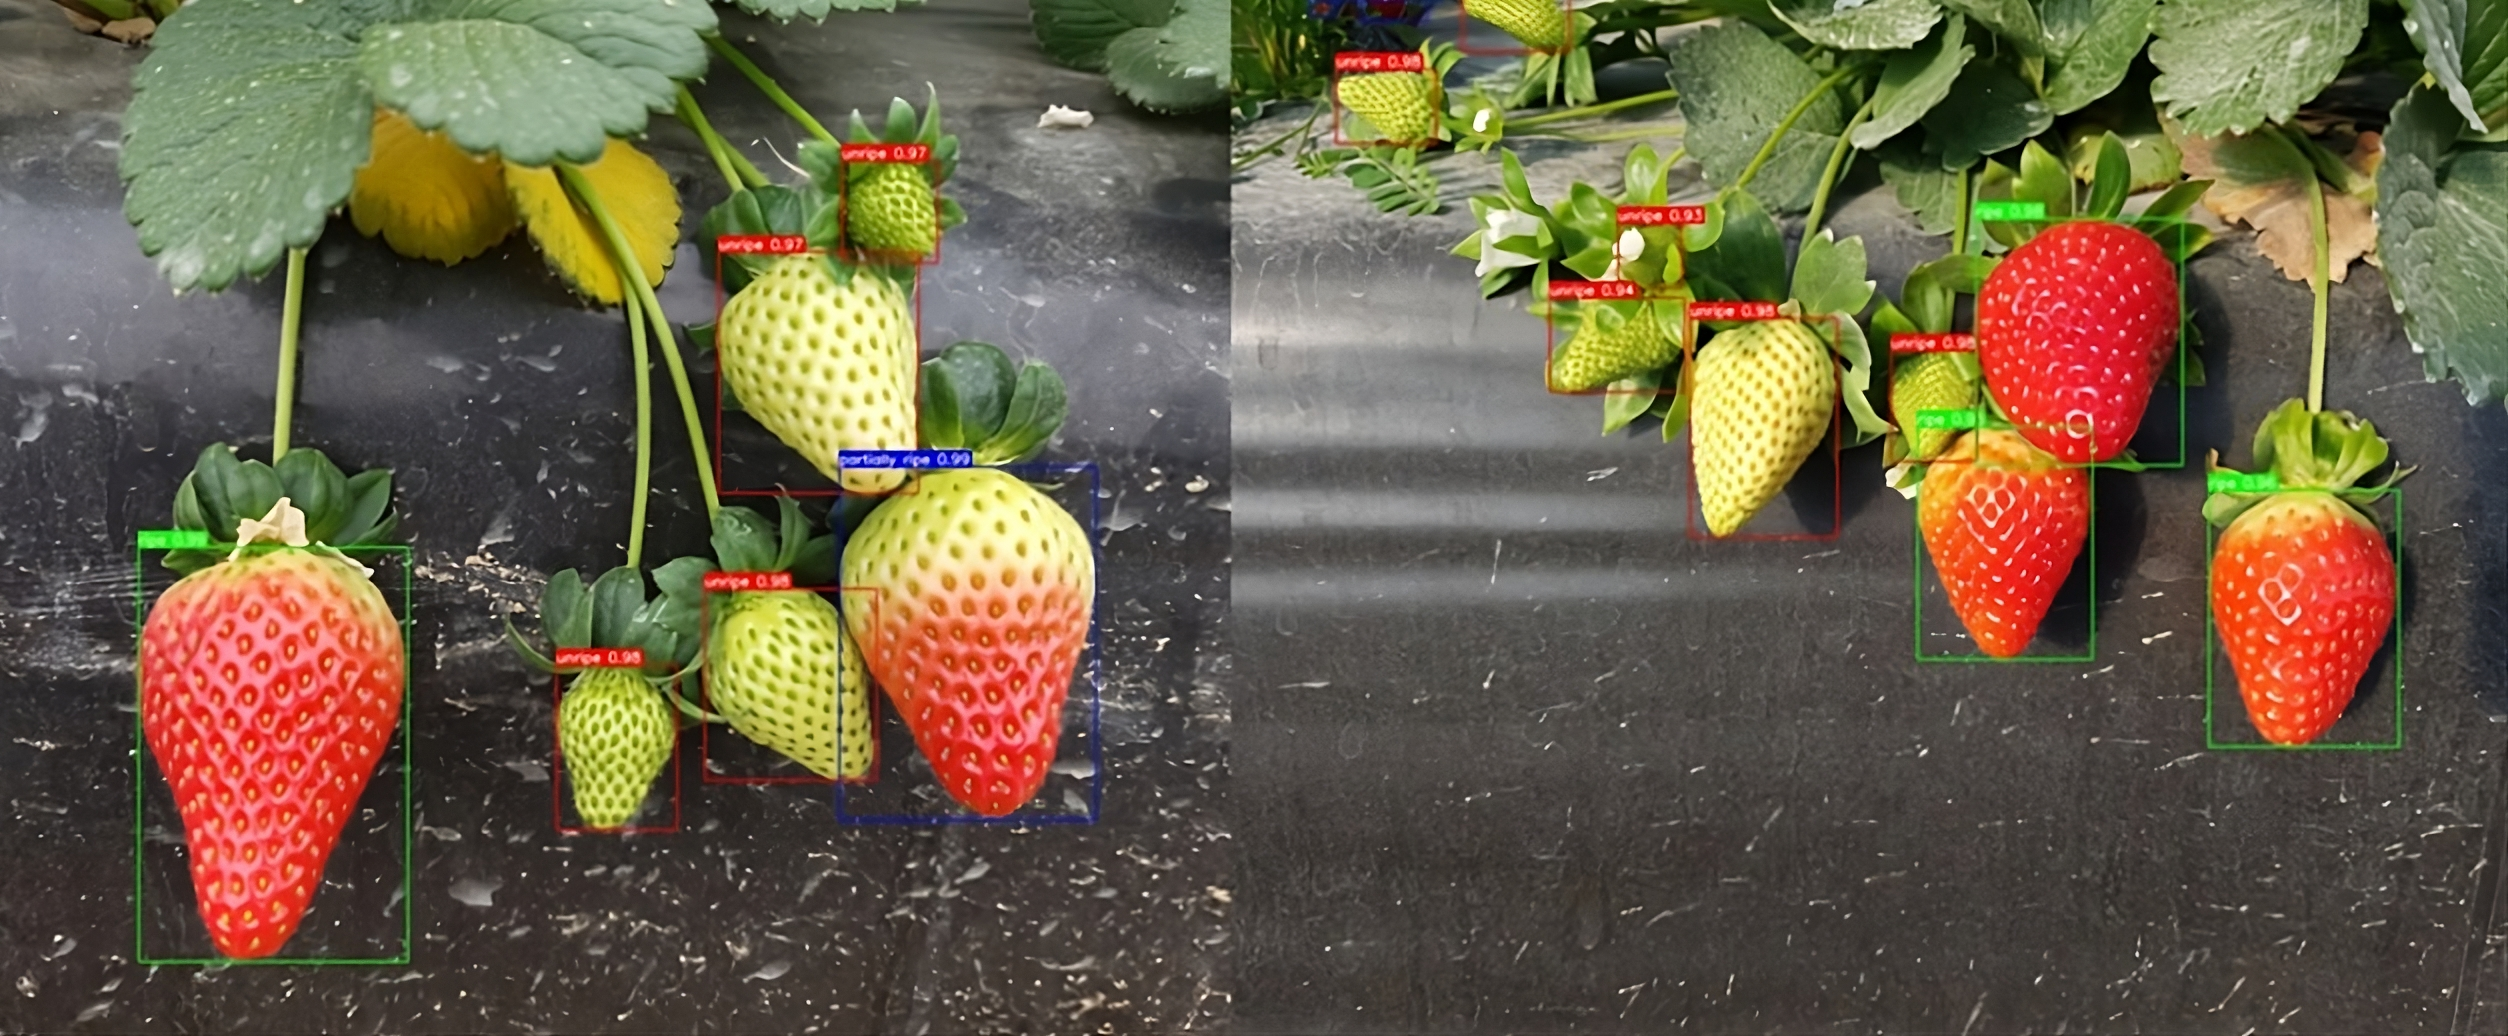
\includegraphics[width=0.8\textwidth]{strawberry.png}
    \caption[Voorbeeld objectdetectie.]{\label{fig:strawberry}Een visueel voorbeeld van objectdetectie: groen duidt rijpe aardbeien aan, rood onrijpe en blauw halfrijpe \autocite{Chai2023}.}
\end{figure}

Segmentatie daarentegen gaat een stap verder: elk pixel in de afbeelding wordt toegewezen aan een specifieke klasse, waardoor objecten niet alleen worden geïdentificeerd, maar ook volledig worden ingekleurd op pixelniveau in plaats van met een kader. Als voorbeeld brengt het de exacte verspreiding van een plantenziekte in kaart of onderscheidt het een plant van de achtergrond.
 
Segmentatie biedt een gedetailleerdere visuele interpretatie dan objectdetectie. Er zijn twee vormen van segmentatie: semantische segmentatie en instantiesegmentatie. Bij semantische segmentatie worden alle objecten van eenzelfde categorie in dezelfde kleur gemarkeerd. Instantiesegmentatie daarentegen wijst elk individueel object binnen een categorie een unieke kleur toe. Hierdoor kunnen objecten binnen dezelfde klasse van elkaar worden onderscheiden. Figuur \ref{fig:plants} toont beide vormen van segmentatie.

\begin{figure}
    \centering
    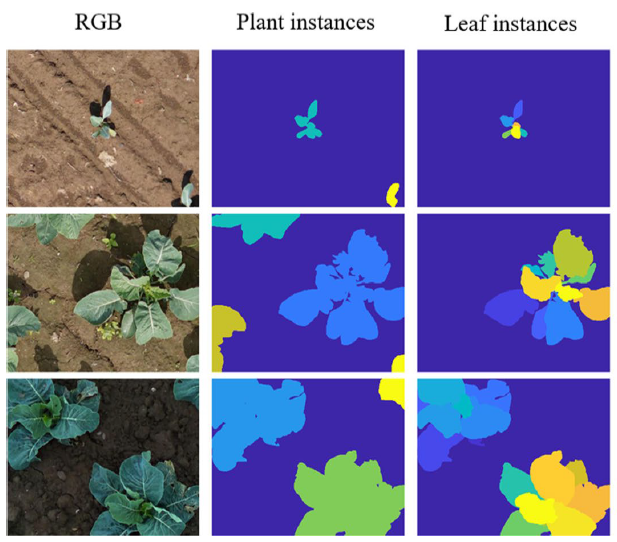
\includegraphics[width=0.85\textwidth]{plants.png}
    \caption[Voorbeeld segmentatie.]{\label{fig:plants}Een visueel voorbeeld van segmentatie. De middelste kolom toont semantische segmentatie van afzonderlijke planten. De rechterkolom geeft instantiesegmentatie weer van individuele bladeren binnen elke plant \autocite{Lei2024}.}
\end{figure}

De proefopstelling van deze bachelorproef bestaat uit een semantisch segmentatiemodel.

\subsection{Huidige uitdagingen}
% EG !!! kritisch zijn (defecten moeten snel en nauwkeurig aangeduid worden, segmentatie heeft veel kracht en opslag nodig ...)







\section{Tips}

Dit hoofdstuk bevat je literatuurstudie. De inhoud gaat verder op de inleiding, maar zal het onderwerp van de bachelorproef *diepgaand* uitspitten. De bedoeling is dat de lezer na lezing van dit hoofdstuk helemaal op de hoogte is van de huidige stand van zaken (state-of-the-art) in het onderzoeksdomein. Iemand die niet vertrouwd is met het onderwerp, weet nu voldoende om de rest van het verhaal te kunnen volgen, zonder dat die er nog andere informatie moet over opzoeken \autocite{Pollefliet2011}.

Je verwijst bij elke bewering die je doet, vakterm die je introduceert, enz.\ naar je bronnen. In \LaTeX{} kan dat met het commando \texttt{$\backslash${textcite\{\}}} of \texttt{$\backslash${autocite\{\}}}. Als argument van het commando geef je de ``sleutel'' van een ``record'' in een bibliografische databank in het Bib\LaTeX{}-formaat (een tekstbestand). Als je expliciet naar de auteur verwijst in de zin (narratieve referentie), gebruik je \texttt{$\backslash${}textcite\{\}}. Soms is de auteursnaam niet expliciet een onderdeel van de zin, dan gebruik je \texttt{$\backslash${}autocite\{\}} (referentie tussen haakjes). Dit gebruik je bv.~bij een citaat, of om in het bijschrift van een overgenomen afbeelding, broncode, tabel, enz. te verwijzen naar de bron. In de volgende paragraaf een voorbeeld van elk.

\textcite{Knuth1998} schreef een van de standaardwerken over sorteer- en zoekalgoritmen. Experten zijn het erover eens dat cloud computing een interessante opportuniteit vormen, zowel voor gebruikers als voor dienstverleners op vlak van informatietechnologie~\autocite{Creeger2009}.

Let er ook op: het \texttt{cite}-commando voor de punt, dus binnen de zin. Je verwijst meteen naar een bron in de eerste zin die erop gebaseerd is, dus niet pas op het einde van een paragraaf.

\begin{figure}
    \centering
    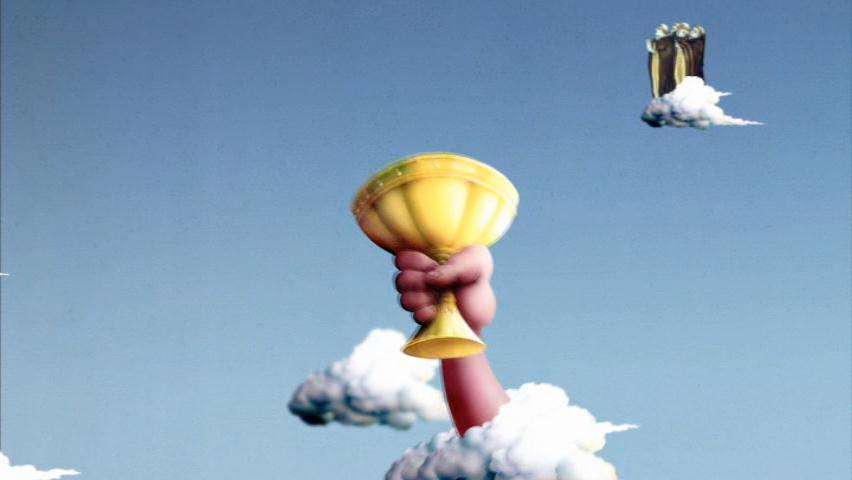
\includegraphics[width=0.8\textwidth]{grail.jpg}
    \caption[Voorbeeld figuur.]{\label{fig:grail}Voorbeeld van invoegen van een figuur. Zorg altijd voor een uitgebreid bijschrift dat de figuur volledig beschrijft zonder in de tekst te moeten gaan zoeken. Vergeet ook je bronvermelding niet!}
\end{figure}